% !TEX root = ../../../thesis.tex
We followed the method outlined in Section~\ref{sec:method-sample-fabrication}. However, in addition to the \ce{Nb} and \ce{Au}, we first sputter a layer of \ce{Cu}. This allows us to make superconductor-normal-superconductor (SNS) junctions. Additionally we used a \ce{Si} wafer with a \qty{300}{\nano\meter} thermal oxide layer. Figure~\ref{fig:CP2.6B-SEM-images} shows the fine structures created using the the FIB. Contrary to the first sample we decided to use a square geometry instead of a circular one. This improves the coupling between the junction loop and the dc-SQUID.

\begin{figure}[ht!]
	\begin{subfigure}[t]{0.3\textwidth}
		\centering
		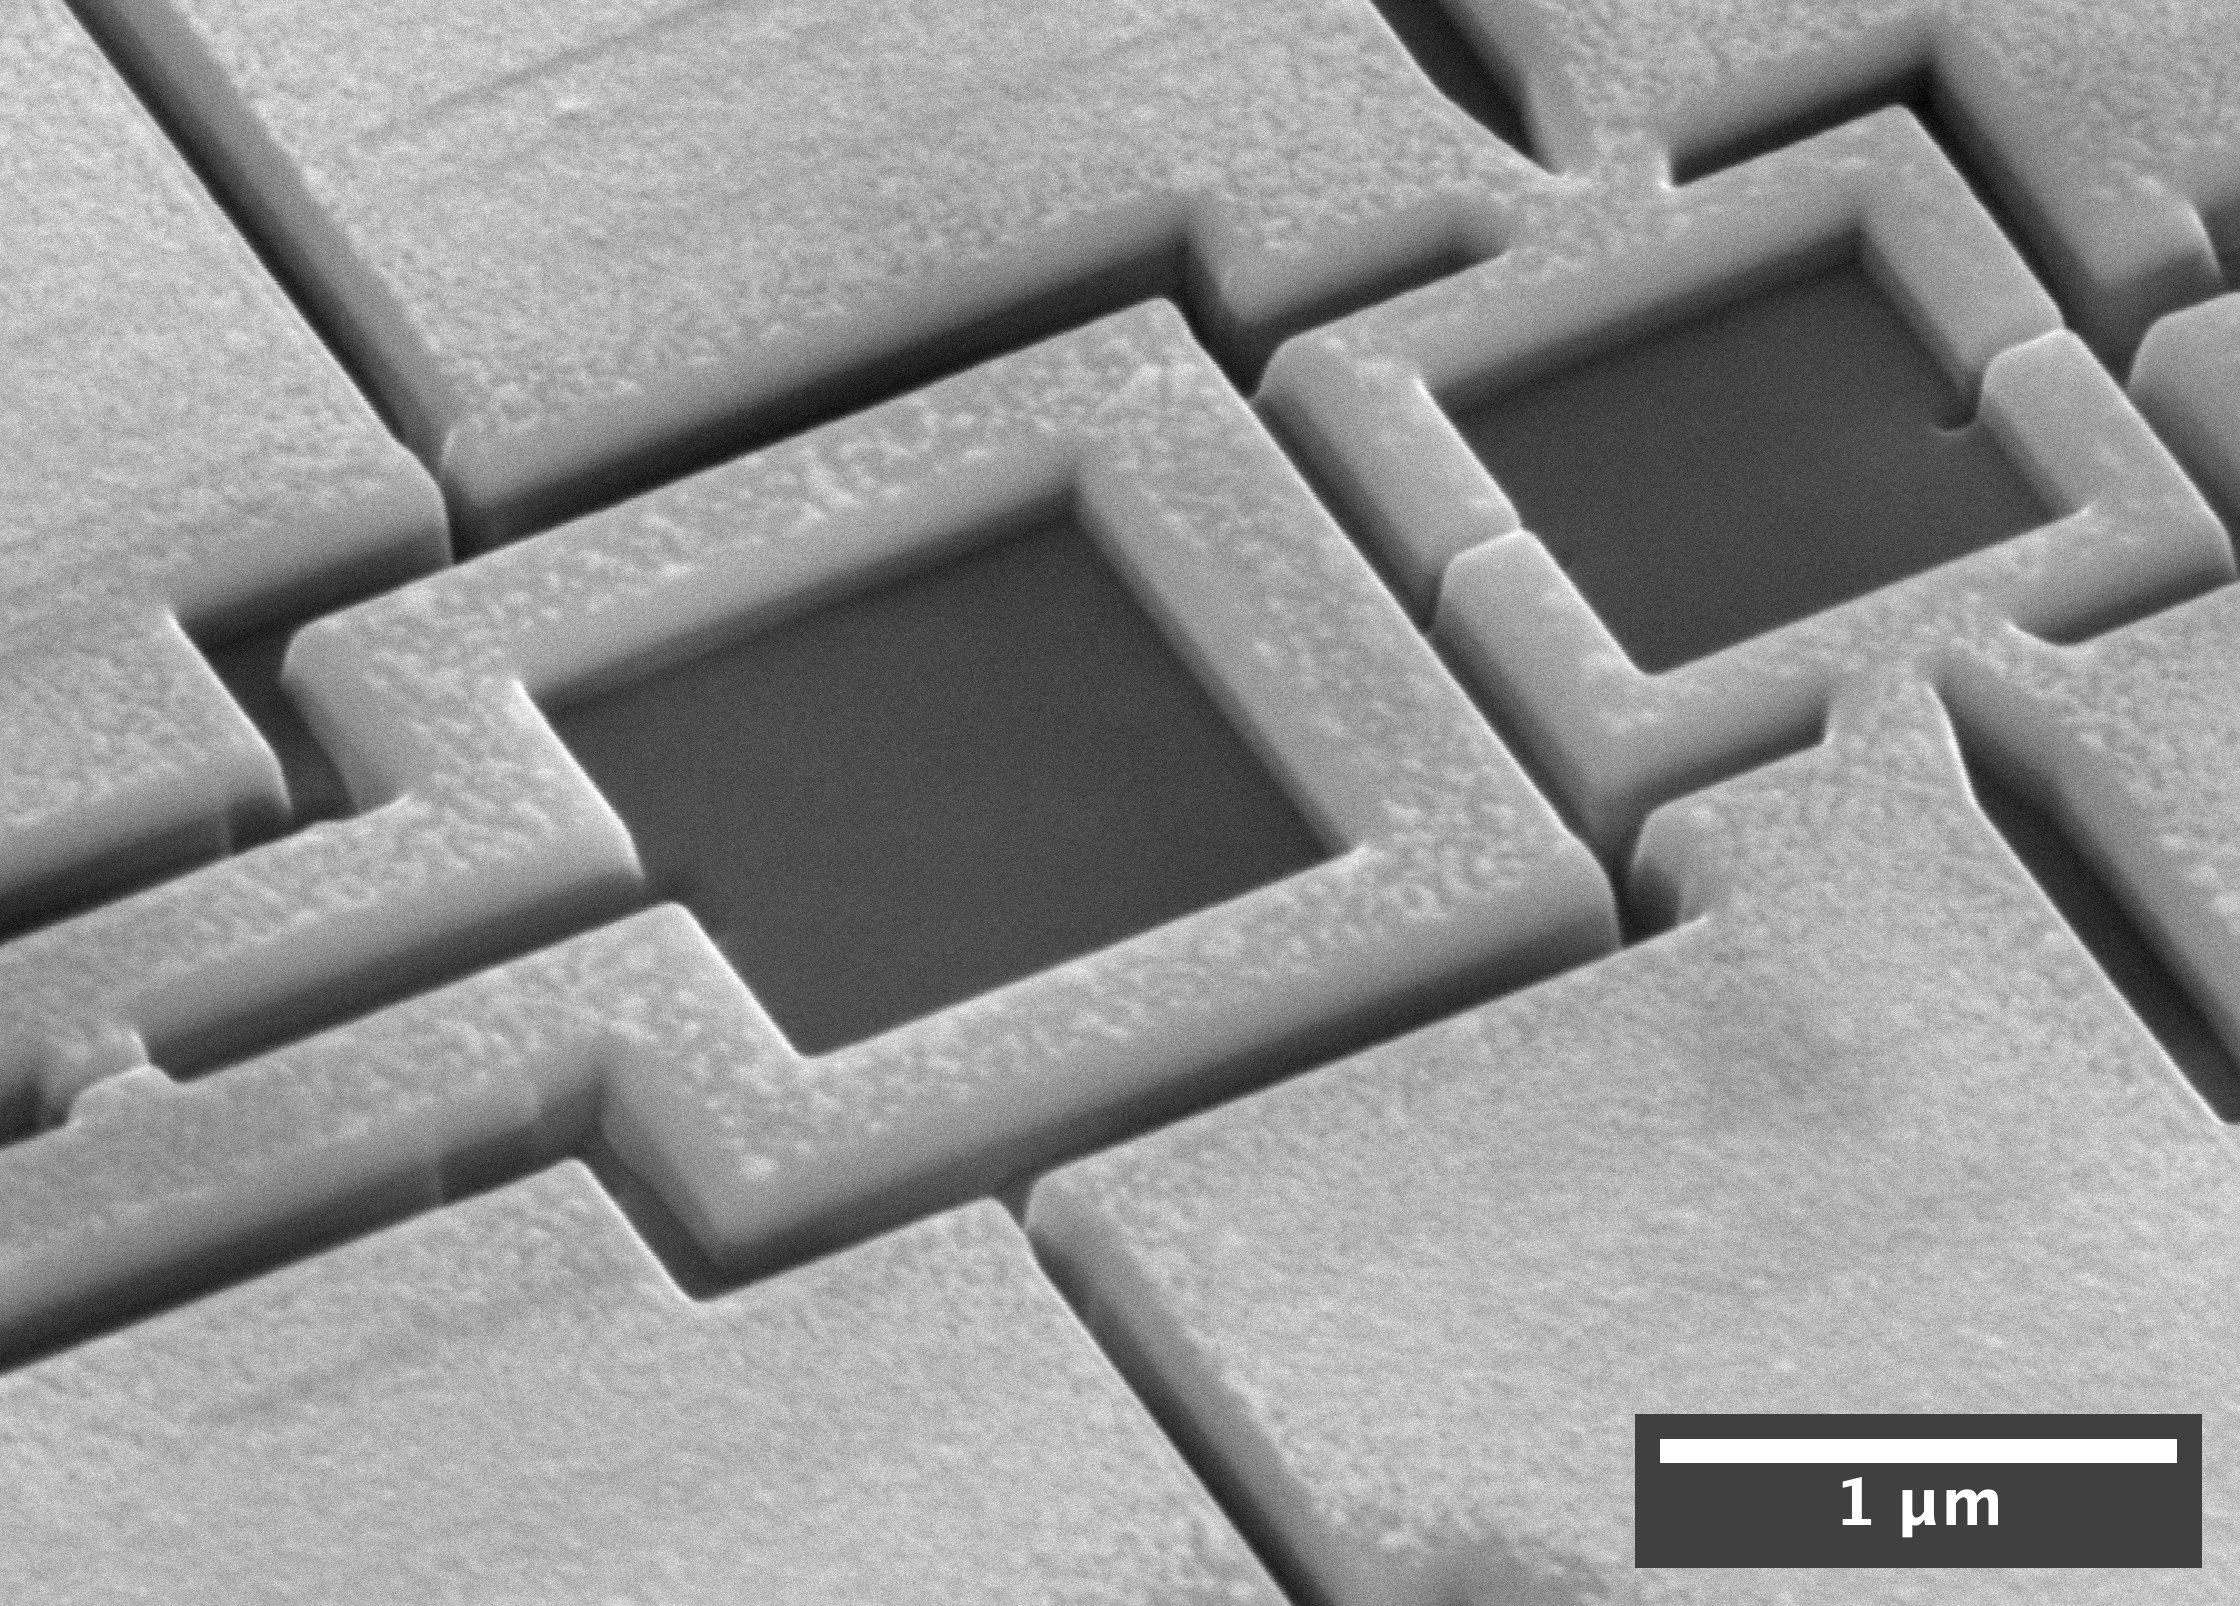
\includegraphics[width=\textwidth]{figures/samples/CP2/CP2.6B_SEM_overview.jpg}
		\subcaption{Overview of the device. The top loop shows the dc-SQUID and the bottom is the junction loop.}
	\end{subfigure}
	\hfill
	\begin{subfigure}[t]{0.3\textwidth}
		\centering
		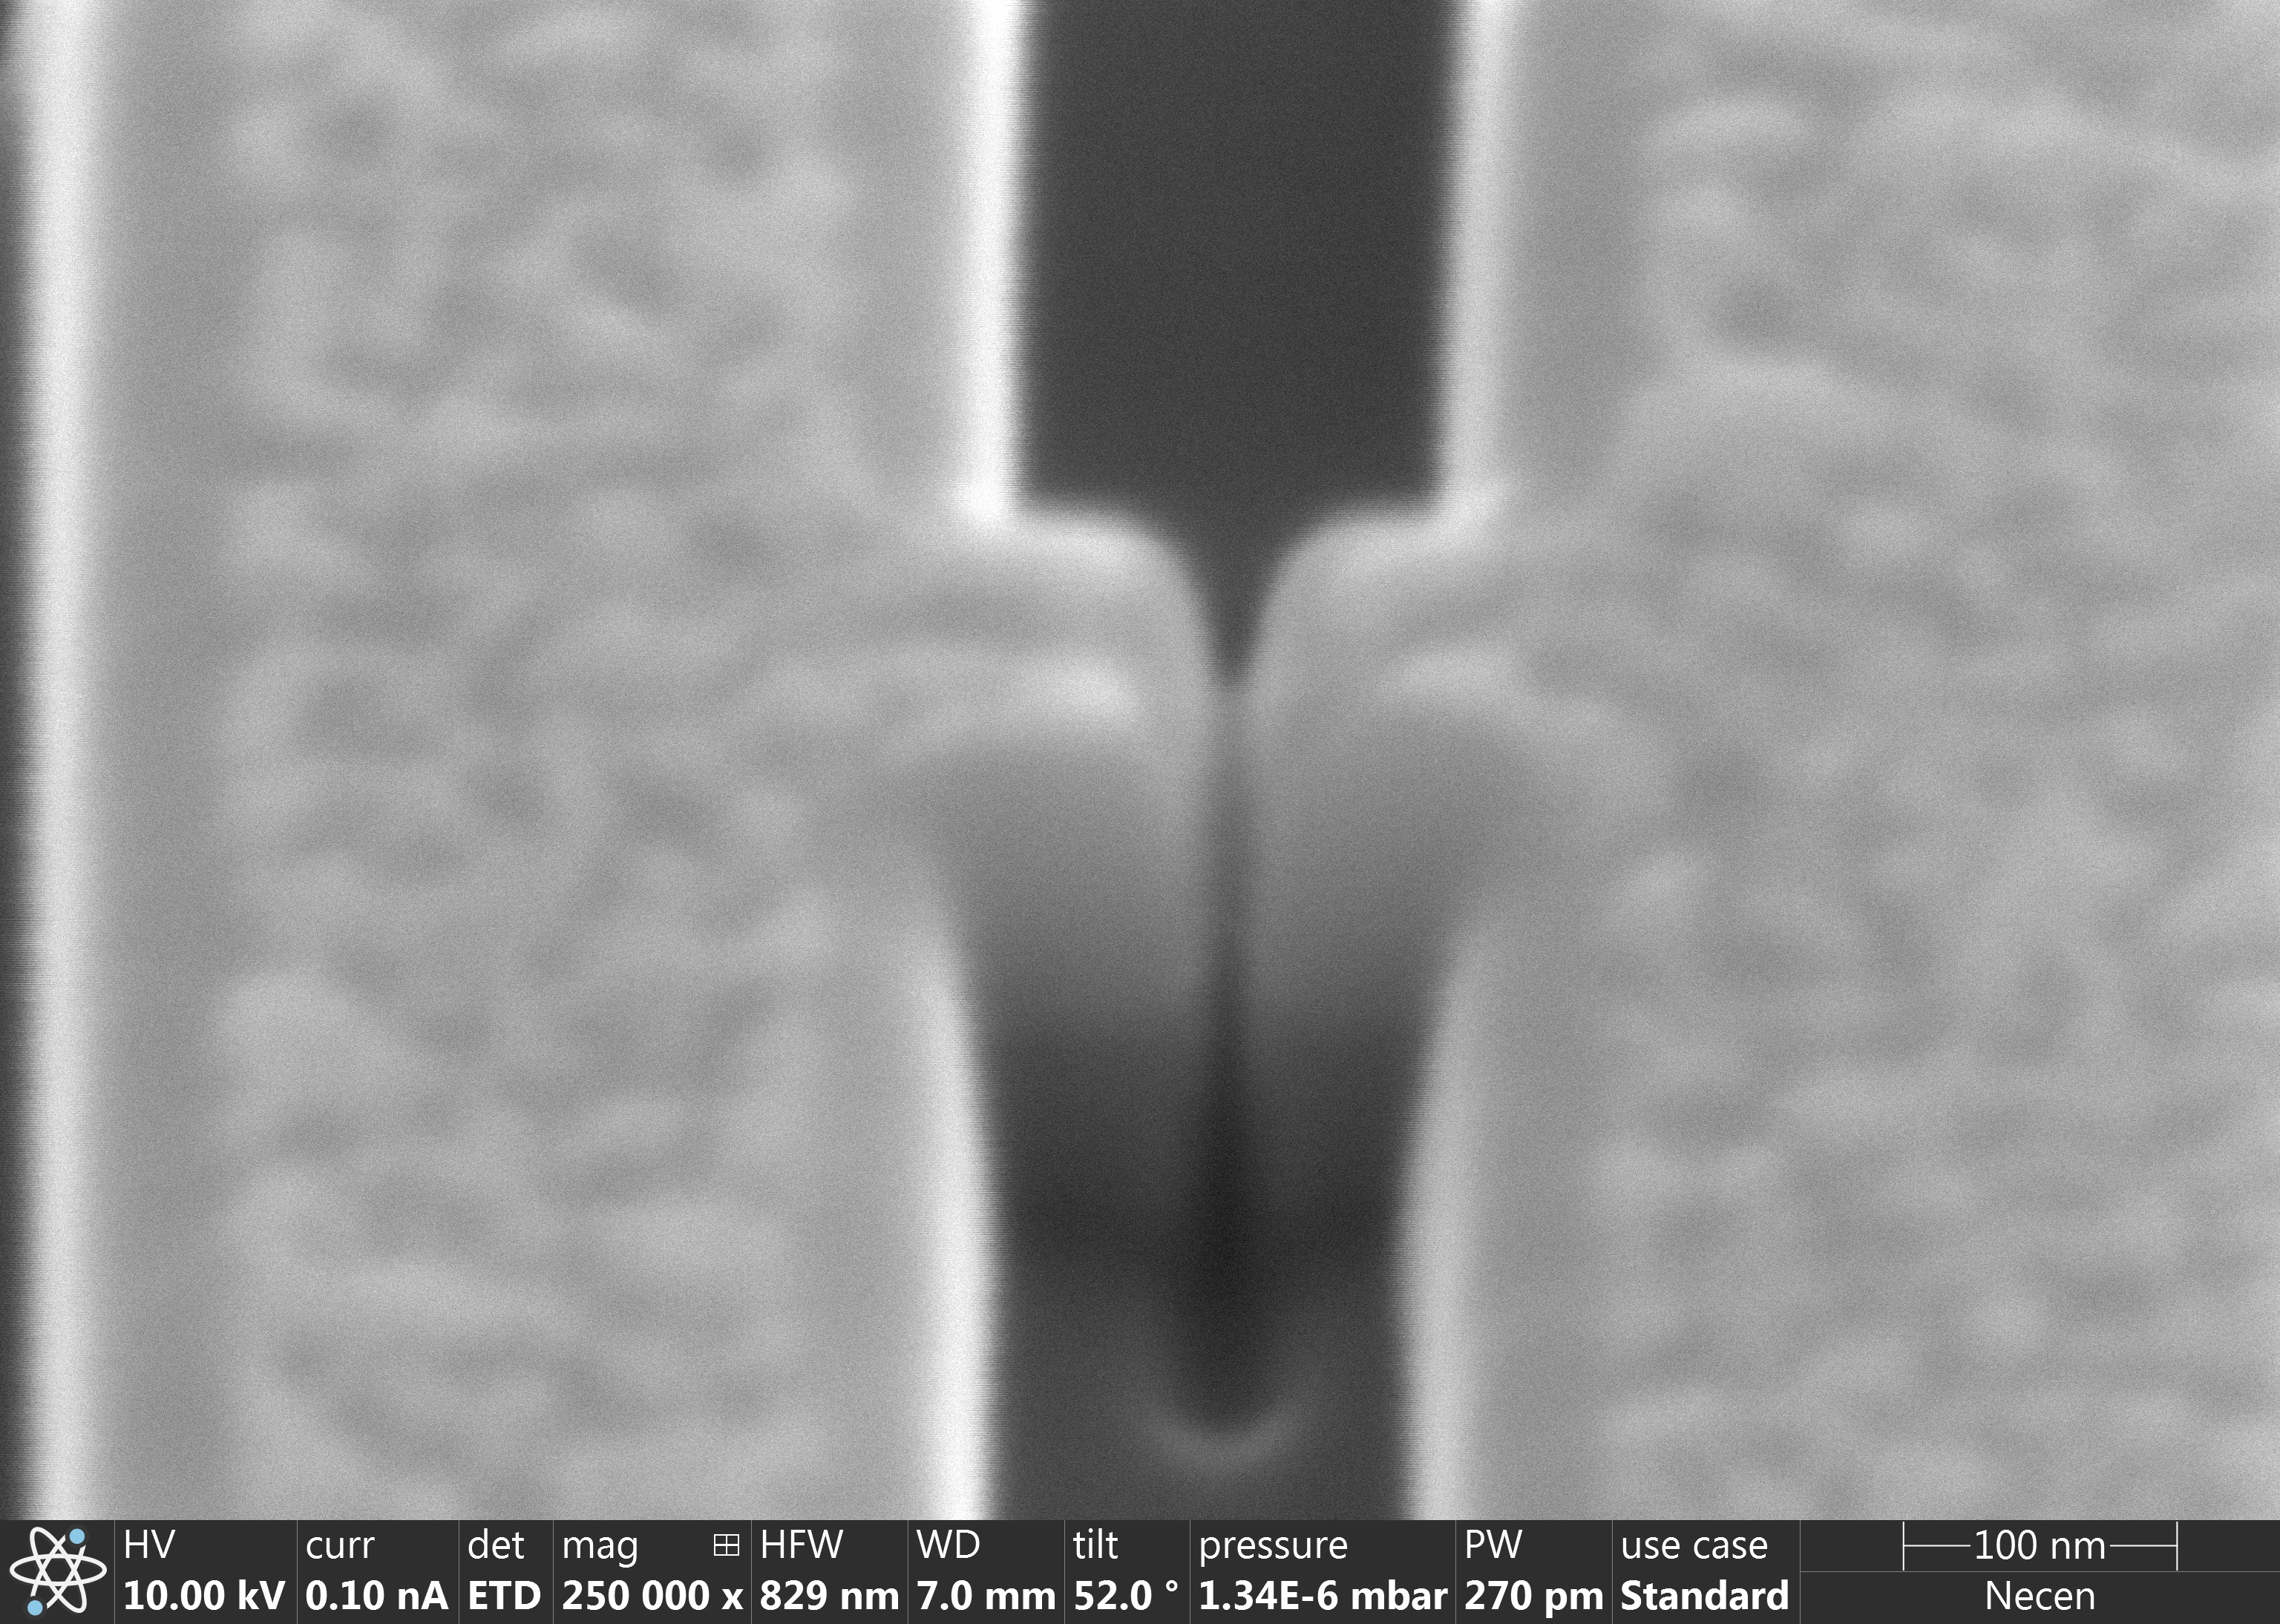
\includegraphics[width=\textwidth]{figures/samples/CP2/CP2.6B_SEM_junction.jpg}
		\subcaption{Zoomed in view of the junction, the width of the junction is \qty{12}{\nano\meter}.}
	\end{subfigure}
	\hfill
	\begin{subfigure}[t]{0.3\textwidth}
		\centering
		\includegraphics[width=\textwidth]{figures/samples/CP2/CP2.6B_SEM_SQUID.jpg}
		\subcaption{Zoomed in view of the dc-SQUID. The width of the junctions is \qty{22}{\nano\meter}.}
	\end{subfigure}

	\caption{Fine structures of sample CP2.6B after the FIB. See Table~\ref{tab:CP2.6B-geometries} for the exact geometries of the sample.}
	\label{fig:CP2.6B-SEM-images}
\end{figure}

\begin{table}
	\begin{subtable}{.6\linewidth}
		\begin{tabular}[t]{@{}lrr@{}}
			\toprule
			Parameter & Value \\ \midrule
			\expandableinput tables/geometries/CP2.6B.tex
			\bottomrule
		\end{tabular}
    \end{subtable}
    \hfill
    \begin{subtable}{.3\linewidth}
    	\flushright
    	\begin{tabular}[t]{@{}lrr@{}}
    		\toprule
    		Parameter & Value \\ \midrule
    		\expandableinput tables/parameters/CP2.6B.tex
    		\bottomrule
    	\end{tabular}
    \end{subtable}
    \caption{The \textbf{left} table provides an overview of the geometries of CP2.6B as determined by SEM imaging and sputtering rates. The \textbf{right} table gives an overview of parameters found using a simulation based on the geometries. The geometries are based on sample CP1.2H.}
    \label{tab:CP2.6B-geometries}
\end{table}